\scanpage{66}
\begin{center}Commentaires Exp. X\end{center}

p.1, li.3 : référence pour $K.(X)$ : (IV 2.2 et 2.4).

p.1, li.15 : non nulle (sans trait d'union).

p.2, li.3 : référer à (EGA IV 3.1.4) pour le fait que $\operatorname{long}(\underline{F}_x)$ est finie.

p.2, li.8 : Prouver l'assertion ``Evidemment $K'$ contient ...'', il y a une petite suite exacte à écrire.

p.2, li.7 du bas : ``On sait (IV 2.11.1) ... ''

p.3, li.5 : (IV 1.4.1 et 2.11.1).

\deleted{p.3, li.7\unsure{:}}

p.3, li.13 : \deleted{référence pour $K$} ajouter ``,noté $K^{\bullet}(X)_{\text{naïf}}$ dans (IV 2.2).''

p.3, li.14 : \deleted{(VI} (VI 3.2) si $X$ est quasi-compact, sinon ?

p.3 : Vider (1.2.1) et (1.2.2).

p.3, li.4 du bas : ``Rappelons (V 3.10) ...''

p.4, li. 3 : ``On a démontré (loc. cit.) ...''

p.4, li.9 : ``Rappelons (IV 2.10) ...''

p.4, li.8 du bas : numérotation canulée pour le Cor. 1.3.3. Peut-être vaut-il mieux , dans l'énoncé de ce corollaire, remplacer $X$ par \inserted{une autre lettre, $Z$ par exemple,} ce qui permettrait de préciser à la ligne du bas : ``tout sous-schéma intègre fermé $Z$ de $X$ ...''
\figure{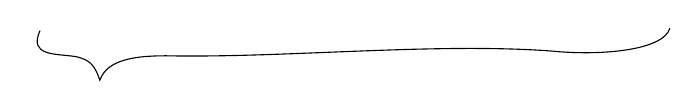
\begin{tikzpicture}
\draw (-4,.28) .. controls (-4.15,-.05) and (-3.8,-.01) .. (-3.55,-.05) .. controls (-3.35,-.09) and (-3.3,-.18) .. (-3.24,-.35) .. controls (-3.15,-.09) and (-2.8,-.04) .. (-2.4,-.04) .. controls (-.9,-.07) and (1.02,.13) .. (2.5,.02) .. controls (3.1,-.04) and (3.91,.02) .. (4,.31);
\end{tikzpicture}}

p.5, li.4 : ``Pour \deleted{\unsure{évitéer}} éviter toute confusion,...''

p.5, li.6 : (IV 2.11.1.2) .

p.5, li. 8 : référence \inserted{\handwritten{(V ...)}} pour $\handwritten{\alpha}^{\unsure{\deleted{x}|\deleted{i}|*|x}}(x)\handwritten{\in}\operatorname{Filt}^{i}(Z)$ .
\figure{\begin{tikzpicture}
\draw (-1,.2) .. controls (-1.08,-.08) and (-.63,-.08) .. (-.24,-.13) .. controls (-.05,-.14) and (.05,-.17) .. (.11,-.42) .. controls (.26,-.23) and (.51,-.16) .. (.76,-.15) .. controls (1.12,-.14) and (1.36,.01) .. (1.39,.31);
\end{tikzpicture}}

p.6, li.1 : (V 3.11 (ii)) .

p.6, li. 6 du bas : ``on peut trouver (cf. VI 4.1) ...''

p.8, li. 1 et 2 du bas : références pour ``universellement caténaire'' et ``Cohen-Macaulay'' ((EGA IV 5.6.3), (EGA IV 5.7.1)). \handwritten{\deleted{\unsure{Voir|Vider|Vides}}}

\handwritten{référence pour l'assertion entre parenthèses \deleted{\unsure{?|:}} (EGA $\overline{\underline{\mathrm{IV}}}$ 6.3.7)}
% archive sheet number: 65
